
\documentclass[12pt,article]{memoir}

\usepackage{fancyhdr}
\usepackage{graphicx}
\usepackage{fontspec}
\setmainfont{Calibri}
\usepackage{tikz}
\usetikzlibrary{calc}
\usepackage{xcolor}
\usepackage{xpatch}
\usepackage{hyperref}

\usepackage{fancyhdr}
\usepackage{graphicx}
\usepackage{fontspec}
\setmainfont{Calibri}
\usepackage{tikz}
\usetikzlibrary{calc}
\usepackage{xcolor}
\usepackage{xpatch}
\usepackage{hyperref}
\usepackage{tabu}
\usepackage{float}
\usepackage[autostyle, english = american]{csquotes}


\usepackage[yyyymmdd]{datetime} % change date format to yyyy/mm/dd to fit ISO8601

\renewcommand{\familydefault}{\sfdefault} % set font
\renewcommand{\dateseparator}{--} % change date-seperators to - to fit ISO8601

\renewcommand\contentsname{Table of Contents}

\chapterstyle{section}
\renewcommand*{\chapnumfont}{\normalfont\HUGE\bfseries\sffamily}
\renewcommand*{\chaptitlefont}{\normalfont\HUGE\bfseries\sffamily}

\makeatletter 
% define macro for itemcode
\newcommand\itemcode[1]{\renewcommand\@itemcode{#1}}
\newcommand\@itemcode{}

% define macro for rev number
\newcommand\revnumber[1]{\renewcommand\@revnumber{#1}}
\newcommand\@revnumber{}
\makeatother

\definecolor{orbitOrange}{RGB}{250,62,0} % the ORBiT orange

\setlrmarginsandblock{2.5cm}{2.5cm}{*}
\setulmarginsandblock{2.5cm}{*}{1}
\checkandfixthelayout 

\setlength{\beforechapskip}{0cm} % reduce chapter spacing

\hypersetup{
    colorlinks,
    citecolor=black,
    filecolor=black,
    linkcolor=black,
    urlcolor=black
}

%**********************************************************************
%Document titles etc. defined here: (replace [] as well)
\title{ORBiT Avionics II System Architecture}
\author{Jinzhi Cai}
\itemcode{Sys-Arch}
\revnumber{A01}
\date{\today}
%end of document titles etc.
%**********************************************************************

\makeatletter
\let\runtitle\@title
\let\runitemcode\@itemcode
\makeatother

% set header style
\pagestyle{fancy}
{
	\fancyheadoffset{0cm}

	\lhead{\runtitle \ - \runitemcode}
	\rhead{Page: \thepage }
	%\chead{\leftmark} % section name
}

\newcommand{\OrbitBackground}{% For a logo drawn with TikZ
\begin{tikzpicture}[remember picture,overlay] % draw background
	\coordinate (bl) at (current page.south west);
	\coordinate (r) at (current page.east);
    \coordinate (A) at ($(bl)+(0,3cm)$);
    \coordinate (B) at ($(r)+(0,-2cm)$);
    \coordinate (C) at (current page.south east);
    \coordinate (ctrlNode) at ($(current page.south) + (0cm,1cm)$);
    \coordinate (ctrlNode2) at ($(current page.south east) + (-1cm,1cm)$);
    \fill[orbitOrange, fill opacity=0.2]
    (A) .. controls (ctrlNode) and (ctrlNode2) .. (B) -- (C) -- (bl);
    \node [white] at ($(C) + (-3cm,1cm)$) {2015-\the\year \ ORBiT@SU};
\end{tikzpicture}
}

\cfoot{\OrbitBackground}

\begin{document}

\begin{tikzpicture}[remember picture,overlay] % draw background
	\coordinate (bl) at (current page.south west);
	\coordinate (r) at (current page.east);
    \coordinate (A) at ($(bl)+(0,3cm)$);
    \coordinate (B) at ($(r)+(0,-2cm)$);
    \coordinate (C) at (current page.south east);
    \coordinate (ctrlNode) at ($(current page.south) + (0cm,1cm)$);
    \coordinate (ctrlNode2) at ($(current page.south east) + (-1cm,1cm)$);
    \fill[orbitOrange]
    (A) .. controls (ctrlNode) and (ctrlNode2) .. (B) -- (C) -- (bl);
    \node [white] at ($(C) + (-3cm,1cm)$) {2015-\the\year \ ORBiT@SU};
\end{tikzpicture}

\makeatletter
	
\includegraphics[width=\textwidth]{../logo.jpg}\\[4ex]
	\begin{center}
	{\fontsize{50}{60}\selectfont \bfseries  \@title }\\[2ex] 
	{\LARGE  \@itemcode}\\
	\end{center}
	\begin{flushright}
	\vspace*{\fill}
	{\LARGE Rev: \@revnumber}\\[2ex]
	{\large \@author}\\[2ex]
	{\large \@date}\\[20ex]
	\end{flushright}
\makeatother
\thispagestyle{empty}
\newpage

\tableofcontents*
\thispagestyle{fancy}
\newpage

%**********************************************************************
% Everything after this is the main document. Edit below this line,
\chapter{ORBiT Avionics II General Software System Architecture}
The software system for OA-II can be divided to three layer: physics layer, system layer, and application layer.
\begin{figure}[htp]
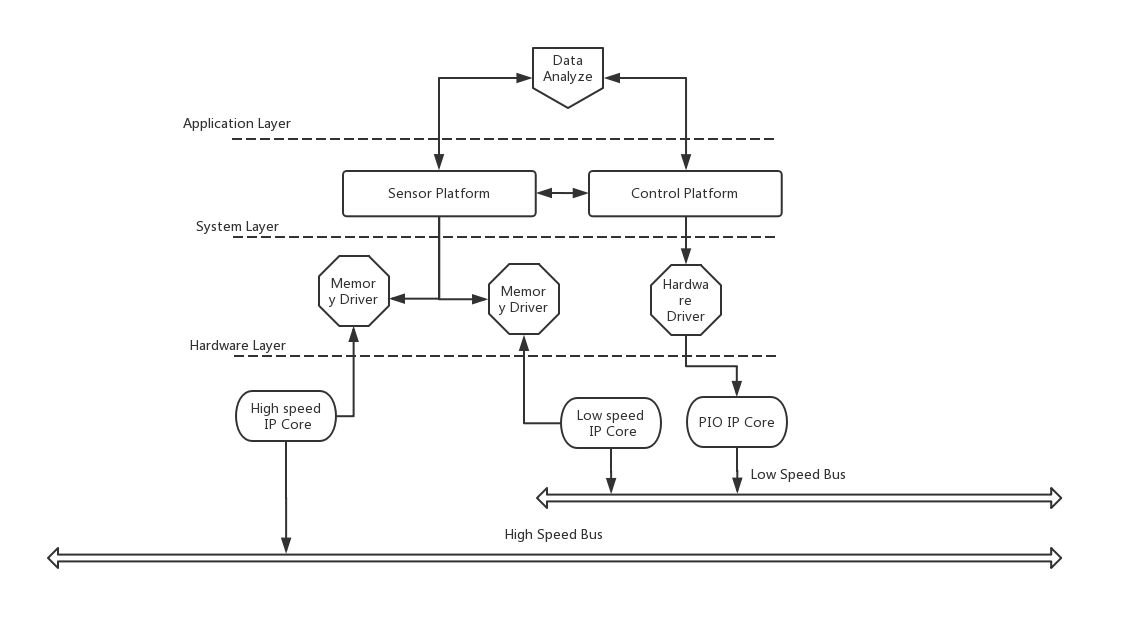
\includegraphics[width=\textwidth]{softarch.png}
\caption{Software Architecture}	
\end{figure}
\section{Physics Layer}
The physics layer program is program that directly interact with hardware memory. It include driver for different buses. It also include the program that directly execute on processor.
\section{System Layer}
The system layer program is program what connect between physics level and application level. It receive data from different physics layer source and group them. It will feed all the grouped data to relative application program. It also provide critical control before and during the fly. In the same time, it also record all the data to on board storage.
\section{Application Layer}
The application layer program is use to process data that provided by the system and provide infomation that will send back to OA-II BAS.\\
\chapter{ORBiT Avionics II General Hardware System Architecture}
\section{Payload Catalogue}
\subsection{Critical Payload} - It is the most important payload which provide data for launch and landing. It will not operating in very high speed, so EMC require will be minimum. It will directly attach to the Swappable Computing Module (SCM). Any of them fail will lead to the cancelation of launch.
\begin{itemize}
\item GPS receivor
\item Battery sensor
\item Low speed IMU
\item Storage media
\item Radio system
\end{itemize}
\subsection{High Speed Payload} - It is the major part of the OA-II payload system. It include the sensor that will collect data conduct futher research. Most of those sensor will be running at $10kHz$ with high standard EMC requirement. It will locate at the Swappable Telemetering Module (STM).
\begin{itemize}
\item Camera
\item Air pressure sensor
\item Other high speed sensor
\end{itemize}
\subsection{Low Speed Payload} - It is the minor part of the OA-II payload system. It contain non-research related sensor and actuator related component. \textit{It might be conatin EMI source.}
\begin{itemize}
\item Actuator
\item TBD
\end{itemize}
\begin{figure}[htp]
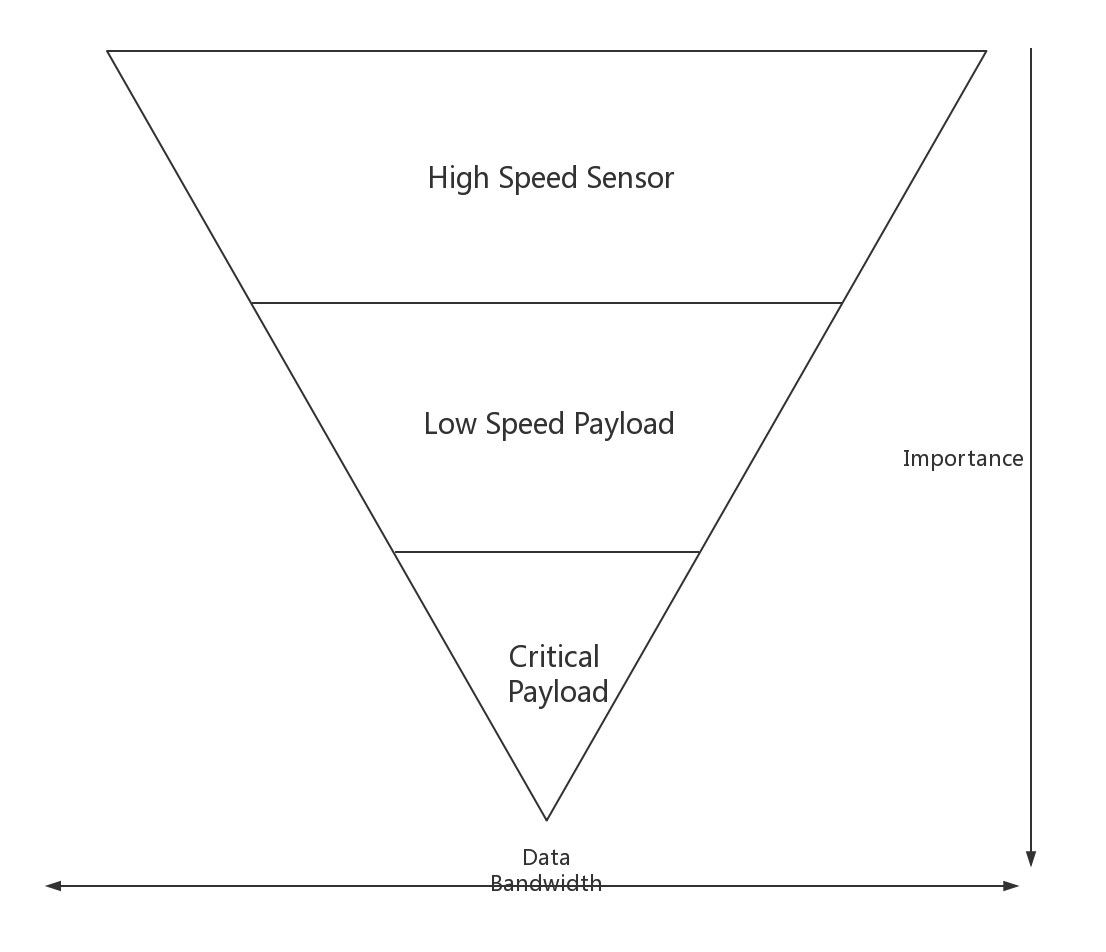
\includegraphics[width=\textwidth]{payloadCata.png}
 \caption{Payload Diagram}	
\end{figure}
\section{PCB Layout}
\section{High Speed Lane Protection}
%*************************************************************************************
%*************************************************************************************
%*************************************************************************************
\chapter{ORBiT Avionics II Vehicle Electronics (OA-II VEH) System Architecture}
\section{General Description}
\section{Mission Module Container (MMC)}
The Mission Module Container (MMC) is use to contain all the Swappable Mission Module (SMM) and provide a high speed bus controller and power supply. The MMC should be a four layers board. The second layer should be use to route high speed traces and the first and third layer be signal ground.
\section{Swappable Mission Module (SMM)}
The Swappable Mission Module (SMM) is a highly specialize circuit that perform special job during and after whole mission. It majorly can be divided to three kinds of SMM, Swappable Computing Module (SCM), Swappable Telemetering Module (STM), Swappable Actuator Module (SAM).\\\\
\subsection{Swappable Computing Module (SCM)}
The Swappable Computing Module (SCM) is use to collecting data from Swappable Telemetering Module (STM). In the same time, it also in charge of the rocket status analyze and control. SCM will determine the status of the rocket and provide emergent countermeasure. SCM also have data storage for future analyze.\\\\
%*****************************************************************************
\subsection{Swappable Telemetering Module (STM)}
The Swappable Telemetering Module (STM) is providing sensing ability and wireless communication with OA-II BSP. The STM system include most of the high speed sensor and low speed sensor, and it provide FIFO buffer for high speed sensor.\\\\
%*****************************************************************************
\subsection{Swappable Actuator Module (SAM)}%Use for landing?
TBD
%\subsection{Adaptable Rockets}
%\section{PCB Layout Description}%\section{PCB Layout and Manufacture Description}
%\subsection{PCB Layout}
%\subsection{PCB Manufacture Requirement}
%***************************************************************************
%**********************************************************************
%**********************************************************************
\chapter{ORBiT Avionics II Base Station Electronics (OA-II BAS) System Architecture}
\section{General Description}
The OA-II BAS is a modulized launch pad and fly control center. It include three untility module: "Supervisor" launch pad control module, "Adviser" automatic vehicle analysis module, "Demonstrator" live data analysis and display module. All of those three 
\section{"Supervisor" Launch Pad Control Module}
The "Supervisor" Launch Pad Control Module is use to manage the rocket status, fuel and oxidizer injection, ignition and cutoff.
\section{"Adviser" Automatic Vehicle Analysis Module}
The "Adviser" Automatic Vehicle Analysis Module use funicle cable to supply power for the vehicle and diagnosing it. It will compare each key value with theoretical value that previous storage in the module and send automatic generated advise to "Demonstrator".
\section{"Demonstrator" Live Data Analysis and Display Module}
The "Demonstrator" Live Data Analysis and Display Module
%***************************************************************************
%**********************************************************************s
\chapter{ORBiT Avionics II Backplane System (OA-II BPS) System Architecture}
\section{General Description}
sadasdasd
\begin{figure}[h]
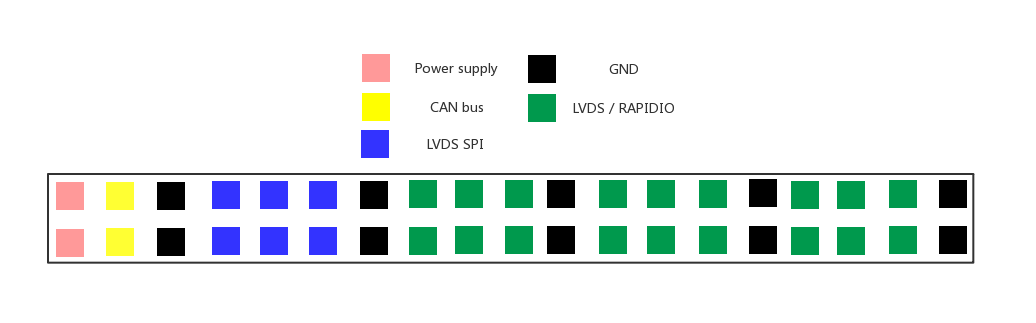
\includegraphics[width=\textwidth]{BPS_Pin.png}
 \caption{Example Pin Out}	
\end{figure}
\section{Software System Structure}
\section{Hardware System Structure}
%\section{System Description}
%\section{Backplane Connection Protocal}
%\subsection{Connection Protocal}
%\subsection{Pin Diagram}
%***************************************************************************
\chapter{ORBiT Avionics II Wireless System (OA-II WLS) System Architecture}
\section{General Description}
\subsection{High Speed Wireless Connection Protocal}
\subsection{Low Power Wireless Connection Protocal}

%\section{System Description}
%\section{}
%\section{}
%end of document
%**********************************************************************
\end{document}

%\begin{table}[H]
%	\centering
%	\begin{tabu}{r || c | c  }
%		Rocket Series & Part Number & Date\\ \hline
%		 ?& ?& ?\\
%		 & & \\
%		 & & \\ 
%		 & & \\
%	\end{tabu}
%	\caption{Adaptable Rockets}
	%\label{tab:edatools}
%\end{table}
%
